\begin{dang}{Góc giữa đường thẳng và mặt phẳng}
	\begin{dn}
		\begin{itemize}
			\item Nếu đường thẳng $a$ vuông góc với mặt phẳng $(P)$ thì ta nói rằng góc giữa đường thẳng $a$ và mặt phẳng $(P)$ bằng $90^{\circ}$.
			\item 	Nếu đường thẳng a không vuông góc với mặt phẳng $(P)$ thì góc giữa a và hình chiếu $a'$ của nó trên $(P)$ được gọi là góc giữa đường thẳng a và mặt phẳng $(P)$.
		\end{itemize}
	\end{dn}
	\begin{tabular}{cc}
		\begin{tikzpicture}[scale=.6,font=\footnotesize,line join=round,line cap=round,>=stealth]
			\path 
			(0,0)coordinate(A) 
			(7,0)coordinate(B) 
			(60:3.5)coordinate(C) 
			($(B)+(C)-(A)$) coordinate(D)
			(3.5,4.5) coordinate(M) 
			(3.5,-1) coordinate(N) 
			(3.5,1.5) coordinate(K) 
			(intersection of M--N and A--B) coordinate(O)		 
			;
			\draw (C)--(A)--(B)--(D)--cycle  
			pic[draw,angle radius=6mm]{angle=B--A--C}
			;
			\draw[red]   (M)--(K) (O)--(N)
			;		
			\draw[dashed,red] (K)--(O);	
			\path (A)+(30:4.5mm)node{$P$}
			(M)+(-30:4mm)node{$a$}
			;
			\fill[black](K)circle(2pt);
		\end{tikzpicture}
		&	\begin{tikzpicture}[scale=.6,font=\footnotesize,line join=round,line cap=round,>=stealth]
			\path 
			(0,0)coordinate(A) 
			(7,0)coordinate(B) 
			(60:3.5)coordinate(C) 
			($(B)+(C)-(A)$) coordinate(D)
			(3.5,4.5) coordinate(M) 
			(3.5,1.5) coordinate(N) 
			(6.5,1.8) coordinate(K) 
			($(K)!1.2!(M)$)coordinate(A1)
			($(K)!1.4!(N)$)coordinate(A2)
			($(M)!1.6!(K)$)coordinate(A3)
			($(N)!1.3!(K)$)coordinate(A4)
			(intersection of M--N and C--D) coordinate(O1)
			(intersection of M--K and C--D) coordinate(O2)
			(intersection of M--A3 and B--D) coordinate(O3)				 
			;
			\draw (C)--(A)--(B)--(D)  (C)--(O1) (D)--(O2)
			(A2)--(N) (M)--(N)--(K)  (K)--(A4)
			pic[draw,angle radius=6mm]{angle=B--A--C}
			pic[draw,angle radius=4mm,double]{angle=M--K--N}
			pic[draw,angle radius=2mm]{right angle=M--N--K}
			;	
			\draw[red] (A1)--(K)  (O3)--(A3);
			\draw[dashed] (O1)--(O2); 
			\draw[dashed,red](K)--(O3);
			\path (A)+(30:4.5mm)node{$P$}
			(A1)+(0:4.5mm)node{$a$}
			(A2)+(40:4.5mm)node{$a'$}
			(M)+(10:4mm)node{$A$}
			(N)+(-90:4mm)node{$H$}
			(K)+(50:4mm)node{$O$}
			;
			\foreach \x in {M,N,K}\fill[black] (\x) circle (1.5pt);
		\end{tikzpicture}
	\end{tabular}\\
	\begin{tabular}{cc}
		\begin{tikzpicture}[scale=.6,font=\footnotesize,line join=round,line cap=round,>=stealth]
			\path 
			(0,0)coordinate(A) 
			(7,0)coordinate(B) 
			(60:3.5)coordinate(C) 
			($(B)+(C)-(A)$) coordinate(D)
			(3.5,4.5) coordinate(M) 
			(3.5,1.5) coordinate(N) 
			(6.5,1.8) coordinate(K)
			($(M)+(K)-(N)$) coordinate(H)
			
			($(H)!1.3!(M)$)coordinate(A1)
			($(M)!1.3!(H)$)coordinate(A2)
			($(K)!1.3!(N)$)coordinate(A3)
			($(N)!1.3!(K)$)coordinate(A4)
			(intersection of M--N and C--D) coordinate(O1)
			(intersection of H--K and C--D) coordinate(O2)			 
			;
			\draw (C)--(A)--(B)--(D)  (C)--(O1) (D)--(O2)
			(A3)--(A4) (M)--(N) (K)--(H)
			pic[draw,angle radius=6mm]{angle=B--A--C}
			pic[draw,angle radius=2mm]{right angle=M--N--K}
			pic[draw,angle radius=2mm]{right angle=H--K--A4}
			;
			\draw[red] (A1)--(A2);
			\draw[dashed] (O1)--(O2);	
			\path (A)+(30:4.5mm)node{$P$}
			(M)+(70:4mm)node{$A$}
			(N)+(-90:4mm)node{$H$}
			(K)+(-90:4mm)node{$K$}
			(H)+(50:4mm)node{$B$}
			(M)--(A1)node[midway,above]{$a$}
			(N)--(A3)node[midway,above]{$a'$}
			;
			\foreach \x in {M,N,K,H}\fill[black] (\x) circle (1.5pt);
		\end{tikzpicture}
		&\begin{tikzpicture}[scale=.6,font=\footnotesize,line join=round,line cap=round,>=stealth]
			\path 
			(0,0)coordinate(A) 
			(7,0)coordinate(B) 
			(60:3.5)coordinate(C) 
			($(B)+(C)-(A)$) coordinate(D)
			(2,1.5) coordinate(M) 
			(6.5,1.8) coordinate(N)
			;
			\draw (C)--(A)--(B)--(D)--cycle  
			pic[draw,angle radius=6mm]{angle=B--A--C}
			;
			\draw[red]  (M)--(N)	;
			\path (A)+(30:4.5mm)node{$P$}
			(M)+(-70:4mm)node{$a'$}
			(N)+(90:4mm)node{$a$}
			;
		\end{tikzpicture}
	\end{tabular}
	\begin{note}
		Chú ý: Nếu $\alpha$ là góc giữa đường thẳng a và mặt phẳng $(P)$ thì $0 \leq \alpha \leq 90^{\circ}$.
	\end{note}
	\begin{nx}
		\immini{Cho điểm $A$ có hình chiếu $H$ trên mặt phẳng $(P)$. Lấy điểm $O$ thuộc mặt phẳng $(P)$, $O$ không trùng $H$. Khi đó góc giữa đường thẳng $A O$ và mặt phẳng $(P)$ bằng góc $AOH$}{\begin{tikzpicture}[scale=.6,font=\footnotesize,line join=round,line cap=round,>=stealth]
				\path 
				(0,0)coordinate(A) 
				(7,0)coordinate(B) 
				(60:3.5)coordinate(C) 
				($(B)+(C)-(A)$) coordinate(D)
				(3.5,4.5) coordinate(M) 
				(3.5,1.5) coordinate(N) 
				(6.5,1.8) coordinate(K) 
				($(K)!1.2!(M)$)coordinate(A1)
				($(K)!1.4!(N)$)coordinate(A2)
				($(M)!1.6!(K)$)coordinate(A3)
				($(N)!1.3!(K)$)coordinate(A4)
				(intersection of M--N and C--D) coordinate(O1)
				(intersection of M--K and C--D) coordinate(O2)
				(intersection of M--A3 and B--D) coordinate(O3)				 
				;
				\draw (C)--(A)--(B)--(D)  (C)--(O1) (D)--(O2)
				(M)--(N)--(K)  
				pic[draw,angle radius=6mm]{angle=B--A--C}
				pic[draw,angle radius=4mm,double]{angle=M--K--N}
				pic[draw,angle radius=2mm]{right angle=M--N--K}
				;	
				\draw (M)--(K)  ;
				\draw[dashed] (O1)--(O2); 
				%	\draw[dashed,red](K)--(O3);
				\path (A)+(30:4.5mm)node{$P$}
				%	(A1)+(0:4.5mm)node{$a$}
				%	(A2)+(40:4.5mm)node{$a'$}
				(M)+(10:4mm)node{$A$}
				(N)+(-90:4mm)node{$H$}
				(K)+(50:4mm)node{$O$}
				;
				\foreach \x in {M,N,K}\fill[black] (\x) circle (1.5pt);
			\end{tikzpicture}
		}
	\end{nx}
	\begin{note}
		\begin{itemize}
			\item Góc $\alpha$ giữa đường thẳng và mặt phẳng luôn thỏa mãn $0^\circ \leq \alpha \leq 90^\circ$.
			\item Nếu đường thẳng $a$ nằm trong $(P)$ hoặc $a$ song song với $(P)$ thì $(a,(P))=0^\circ$. 
		\end{itemize}
	\end{note}
	
\end{dang}
\subsubsection{VÍ DỤ MẪU}
\begin{vd}%[Huỳnh Đức Vũ, soạn đề cương toán 11-KNTT]%[1C8B3-1]
	Cho hình chóp $S.ABC$ có $SA \perp(ABC)$.
	\begin{enumerate}
		\item Tính góc giữa đường thẳng $SA$ và mặt phẳng $(ABC)$ theo đơn vị độ.
		\item  Tính góc giữa đường thẳng $SB$ và mặt phẳng $(ABC)$ theo đơn vị độ, biết $SA=\sqrt{3}AB$.
	\end{enumerate}
	\loigiai{
		\immini
		{
			\begin{enumerate}
				\item  Vì $SA \perp(ABC)$ nên góc giữa đường thẳng $SA$ và mặt phẳng $(ABC)$ bằng $90^\circ$.
				\item Vì $SA \perp(ABC)$ nên $AB$ là hình chiếu của $SB$ trên $(ABC)$. Suy ra góc giữa đường thẳng $SB$ và mặt phẳng $(ABC)$ bằng $\widehat{SBA}$.\\  Vì tan $\widehat{SBA}=\dfrac{SA}{AB}=\sqrt{3}$ nên $\widehat{SBA}=60^\circ$. \\
				Vậy góc giữa đường thẳng $SB$ và mặt phẳng $(ABC)$ bằng $60^\circ$.
			\end{enumerate}
		}
		{
			\begin{tikzpicture}[scale=1, font=\footnotesize, line join=round, line cap=round, >=stealth]
				\path
				(0,0) coordinate (A)
				(4,0) coordinate (B)
				(2,-1) coordinate (C)
				(0,3) coordinate (S)
				;
				\draw (S)--(A)--(C)--(S)--(B)--(C);
				\draw[dashed] (A)--(B);
				\foreach \x/\g in {S/90,A/180,B/0,C/270} \fill[black] (\x) circle (1pt)+(\g:0.3) node{$\x$};
			\end{tikzpicture}
		}
	}
\end{vd}
\begin{vd}%[Huỳnh Đức Vũ, soạn đề cương toán 11-KNTT]%[1H3B3-3]
	Cho hình chóp $S.ABCD$ có đáy $ABCD$ là hình vuông cạnh $a$, cạnh $SA=a\sqrt{6}$ và vuông góc với đáy. Tính
	\begin{enumerate}
		\item Góc giữa đường thẳng $BC$ và $(SAB)$;
		\item Góc giữa đường thẳng $BD$ và $(SAD)$;
		\item Góc giữa đường thẳng $SC$ và $(ABCD)$.
	\end{enumerate}
	\loigiai{	
		\immini{		
			\begin{enumerate}			
				\item Ta có $SA\perp (ABCD)$, suy ra $BC\perp SA$.\\
				Lại có $BC\perp AB$, suy ra $BC\perp (SAB)$.\\
				Suy ra góc giữa đường thẳng $BC$ và $(SAB)$ bằng $90^\circ$.
				\item Ta có $SA\perp (ABCD)$, suy ra $BA\perp SA$.\\
				Lại có $BA\perp AD$, suy ra $BA\perp (SAD)$.\\
				Vậy $AD$ là hình chiếu của của $BD$ trên $(SAD)$. \\
				Nếu gọi $\varphi$ là góc giữa $BD$ và $(SAD)$ thì \\$\varphi = (BD,AD)=\widehat{BDA}=45^\circ$ (vì $\triangle ABD$ vuông cân tại $A$).
				\item Ta có $SA\perp (ABCD)$, suy ra $AC$ là hình chiếu của $SC$ lên $(ABCD)$.\\
				Nếu gọi $\varphi'$ là góc giữa đường thẳng $SC$ và $(ABCD)$ thì $\varphi'=(SC,CA)=\widehat{SCA}$.\\
				Trong $\triangle SCA$ vuông tại $A$, ta có
				$\tan \widehat{SCA}=\dfrac{SA}{AC}=\dfrac{a\sqrt{6}}{a\sqrt{2}}=\sqrt{3}.$\\
				Suy ra góc giữa đường thẳng $SC$ và $(ABCD)$ bằng $60^\circ$.
				
		\end{enumerate}}{	\begin{tikzpicture}[>=stealth,line join=round,line cap=round,font=\footnotesize,scale=0.6]
				\coordinate[label=above left:{$A$}] (A) at (0,0);
				\coordinate[label=below left:{$B$}] (B) at (-2,-1.75);
				\coordinate[label=below right:{$C$}] (C) at (3.5,-1.75);
				\coordinate[label=right:{$D$}] (D) at ($(A)+(C)-(B)$);
				\coordinate[label=above:{$S$}] (S) at (0,4);
				\coordinate (O) at (intersection of A--C and B--D);
				
				\draw (S)--(B)--(C)--(D)--cycle (S)--(C);
				\draw[dashed] (S)--(A)--(B) (A)--(D) (A)--(C) (B)--(D);
				
				\foreach \p in {A,B,C,D,S}
				\fill (\p) circle (1.2pt);
				\foreach \x/\y/\z in {S/A/B,D/A/S,D/O/A}
				\pic[draw,angle radius=2mm,angle eccentricity=1.5] {right angle = \x--\y--\z};
				\pic[draw,angle radius=4mm,angle eccentricity=1.5] { angle = S--C--A};
		\end{tikzpicture}} 
	}
\end{vd}

%Ví dụ 2
\begin{vd}%[Huỳnh Đức Vũ, soạn đề cương toán 11-KNTT]%[1H3B3-3]
	Cho hình lập phương $ABCD.A'B'C'D'$. Tính góc giữa các đường thẳng sau đây với mặt phẳng $(ABCD)$.
	\begin{enumEX}{3}
		\item $AA'$;
		\item $BC'$;
		\item $A'C$.
	\end{enumEX}
	\loigiai{
		\immini{		
			\begin{enumerate}[a)]
				\item Gọi $a$ là độ dài cạnh của hình lập phương đã cho.\\Vì $ABCD.A'B'C'D'$ là hình lập phương nên ta có \\$AA'\perp (ABCD)$. 
				Suy ra $(AA',(ABCD))=90^\circ$.
				\item Ta có $CC'\perp (ABCD)$ nên suy ra $BC$ là hình chiếu của $BC'$ trên $(ABCD)$.\\
				Khi đó $(BC',(ABCD))=(BC',BC)=\widehat{C'BC}$.\\
				Xét $\triangle C'BC$ vuông tại $C$, ta có
				\[\tan \widehat{C'BC}=\dfrac{CC'}{BC}=\dfrac{a}{a}=1\Rightarrow \widehat{C'BC}= 45^\circ .\]
				Vậy $(BC',(ABCD))= 45^\circ $.
				\item Ta có $AA'\perp (ABCD)$ nên suy ra $AC$ là hình chiếu của $A'C$ trên $(ABCD)$.\\
				Khi đó $(A'C,(ABCD))=(A'C,AC)=\widehat{A'CA}$.\\
				Xét $\triangle A'CA$ vuông tại $A$, ta có
				\[\tan \widehat{A'CA}=\dfrac{AA'}{AC}=\dfrac{a}{a\sqrt{2}}=\dfrac{1}{\sqrt{2}}\Rightarrow \widehat{A'CA}\approx 35^\circ 15'.\]
				Vậy $(A'C,(ABCD)) \approx 35^\circ 15'$.
		\end{enumerate}}{\begin{tikzpicture}[>=stealth,line join=round,line cap=round,font=\footnotesize,scale=0.6]
				\coordinate[label=above left:{$A$}] (A) at (0,0);
				\coordinate[label=below left:{$B$}] (B) at (-2.75,-1.5);
				\coordinate[label=right:{$D$}] (D) at (4.5,0);
				\coordinate[label=below right:{$C$}] (C) at ($(B)+(D)-(A)$);
				\coordinate[label=above left:{$A'$}] (A') at (0,4.5);
				\coordinate[label=above right:{$D'$}] (D') at ($(D)+(A')-(A)$);
				\coordinate[label=above left:{$B'$}] (B') at ($(A')+(B)-(A)$);
				\coordinate[label=above left:{$C'$}] (C') at ($(B')+(D')-(A')$);
				
				
				\draw (A')--(B')--(C')--(D')--cycle (B)--(B') (C)--(C') (D)--(D')
				(B)--(C)--(D) (C')--(B);
				\draw[dashed] (A)--(A') (B)--(A)--(D) (A)--(C) (A')--(C);
				
				\foreach \p in {A,B,C,D,A',B',C',D'}
				\fill (\p)	circle (1.2pt);	
		\end{tikzpicture}}
	}
\end{vd}
\subsubsection{BÀI TẬP TỰ LUẬN}
\begin{bt}%[Huỳnh Đức Vũ, soạn đề cương toán 11-KNTT]%[1H3B3-3]
	Cho hình chóp $S.ABCD$ có đáy $ABCD$ là hình vuông cạnh $a\sqrt{3}$, $SA$ vuông góc với mặt phẳng đáy và $SA=a\sqrt{2}$. Tính góc giữa $SC$ và mặt phẳng $(ABCD)$ .
	\loigiai{
		\immini
		{Ta có $SA\perp (ABCD)$ suy ra $\left(SC,(ABCD)\right)=(SC,AC)=\widehat{SCA}$.\\
			Trong $\triangle SAC$ có $\tan \widehat{SCA}=\dfrac{SA}{AC}=\dfrac{a\sqrt{2}}{a\sqrt{6}}=\dfrac{1}{\sqrt{3}} \Rightarrow \widehat{SCA}=30^{\circ}$.\\
			Vậy $\left(SC,(ABCD)\right)=30^{\circ}$.}
		{\begin{tikzpicture}[scale=1, font=\footnotesize, line join=round, line cap=round, >=stealth]
				\def\bc{4}
				\def\ba{2}
				\def\h{4}
				\def\gocB{30}
				\coordinate[label=below left:$B$] (B) at (0,0);
				\coordinate[label=above left:$A$] (A) at (1.2,1);
				\coordinate[label=below:$C$] (C) at (3,0);
				\coordinate[label=right:$D$] (D) at ($(C)-(B)+(A)$);
				\coordinate[label=above:$S$] (S) at ($(A)+(90:2.5)$);
				\draw (B)--(C)--(D)--(S)--cycle (S)--(C);
				\draw[dashed] (C)--(A)--(D) (S)--(A)--(B);
				\draw pic[draw,angle radius=3mm] {right angle = D--A--S};
				\draw pic[draw,angle radius=5mm] {angle = S--C--A};
				\foreach \diem in {A,B,C,D,S}\fill (\diem)circle(1.5pt);
		\end{tikzpicture}}
	}
\end{bt}
\begin{bt}%[Huỳnh Đức Vũ, soạn đề cương toán 11-KNTT]%[1H3K3-3]
	Cho hình chóp $S.ABCD$ có đáy $ABCD$ là hình chữ nhật, $AB=a\sqrt{2}$, $AD=a$, $SA$ vuông góc
	với đáy và $SA=a$. Tính góc giữa $SC$ và $(SAB)$. 
	\loigiai
	{
		\immini
		{
			Từ $\heva{& BC\perp AB \\ & BC\perp SA}\Rightarrow  BC\perp (SAB)$.\\
			Suy ra $SB$ là hình chiếu vuông góc của $SC$ lên $(SAB)$.\\
			Do đó $(SC,(SAB))=(SC,SB)=\widehat{CSB}$.\\
			Vì $CB\perp (SAB)\Rightarrow BC\perp SB$.
			Tam giác vuông $SBC$ có
			\begin{align*}
				\tan \widehat{BSC}=\dfrac{BC}{SB}=\dfrac{AD}{\sqrt{SA^2+AB^2}}=\dfrac{a}{a\sqrt{3}}=\dfrac{\sqrt{3}}{3}\Rightarrow \widehat{BSC}=30^\circ.
			\end{align*}
			Do đó $(SC,(SAB))=30^\circ$.
		}
		{
			\begin{tikzpicture}[line join = round, line cap = round,>=stealth,font=\footnotesize,scale=0.8]
				\def \b{-1.4};
				\def \c{2.5};
				\def \h{3}
				\path
				(0,0) coordinate (A)
				(\b,\b) coordinate (B)
				(\c,\b) coordinate (C)
				($(A)+(C)-(B)$) coordinate (D)
				($(A)+(0,\h)$) coordinate (S)
				;
				\draw[dashed] (S) -- (A) -- (C) (A) -- (B) (A) -- (D) (A);
				\draw (S) -- (B) -- (C) -- (D) -- (S) -- (C);
				\foreach \x/\g in {A/180,B/180,C/0,D/0,S/90} \fill[black](\x) circle (1pt)+(\g:3mm) node{$\x$};
			\end{tikzpicture}
		}
	}
\end{bt}
\begin{bt}%[Huỳnh Đức Vũ, soạn đề cương toán 11-KNTT]%[1H3K3-3]
	\immini{
		Cho hình chóp tứ giác đều $S.ABCD$ có tất cả các cạnh bằng $a$. Gọi $M$ là điểm trên đoạn $SD$ sao cho $SM=2MD$ (tham khảo hình vẽ bên). Gọi $\alpha$ là góc giữa đường thẳng $BM$ và mặt phẳng $(ABCD)$. Tính $\tan\alpha$.
		\choice
		{\True $\dfrac{1}{5}$}
		{$\sqrt{3}$}
		{$1$}
		{$\dfrac{1}{3}$}
	}{
		\begin{tikzpicture}[scale=0.7, font=\footnotesize, line join=round, line cap=round,>=stealth]
			\path
			(0,0) coordinate (A)
			(-1.9,-1.6)coordinate (B)
			(1.6,-1.6)coordinate (C)
			($(A)+(C)-(B)$)coordinate (D)
			($(A)!0.5!(C)$)coordinate (O)
			($(O)+(0,3.5)$) coordinate (S)
			($(S)!2/3!(D)$) coordinate (M)
			;
			\draw (S)--(B)--(C)--(D)--cycle (S)--(C);
			\draw[dashed] (O)--(S)--(A)--(D) (C)--(A)--(B)--(D) (B)--(M);
			\foreach \p/\q in {S/90,A/170,B/-90,C/-90,D/0,M/70}
			\fill[black] (\p) circle (1.0pt)node[shift={(\q:3mm)}]{$\p$};
	\end{tikzpicture}}
	\loigiai{
		\immini{
			Gọi $O=AC\cap BD$, gọi $H$ là hình chiếu của $M$ trên $(ABCD)$.\\
			Suy ra $SO\perp(ABCD)$, $H\in BD$, $MH\perp (ABCD)$ và $DH=\dfrac{1}{3}DO=\dfrac{a\sqrt{2}}{6}$.\\
			Vì tam giác $SAC$ vuông cân tại $A$, $AC =a\sqrt{2}$ nên $SO=\dfrac{a\sqrt{2}}{2}$.\\
			Hình chiếu của $BM$ lên $(ABCD)$ là $BH$.\\
			Do đó $(BM,(ABCD))=(BM,BH)=\widehat{MBH}=\alpha$.\\
			Ta lại có $BH=\dfrac{5}{6}BD=\dfrac{5a\sqrt{2}}{6}$,\\ $MH=\dfrac{1}{3}SO=\dfrac{1}{3}\cdot\dfrac{a\sqrt{2}}{2}=\dfrac{a\sqrt{2}}{6}$.\\
			Trong tam giác $BMH$, ta có $\tan\alpha=\dfrac{MH}{BH} =\dfrac{\dfrac{a\sqrt{2}}{6}}{\dfrac{5a\sqrt{2}}{6}}=\dfrac{1}{5}$.
		}{
			\begin{tikzpicture}[scale=0.8, font=\footnotesize, line join=round, line cap=round,>=stealth]
				\path
				(0,0) coordinate (A)
				(-1.9,-1.6)coordinate (B)
				(1.6,-1.6)coordinate (C)
				($(A)+(C)-(B)$)coordinate (D)
				($(A)!0.5!(C)$)coordinate (O)
				($(O)+(0,3.5)$) coordinate (S)
				($(S)!2/3!(D)$) coordinate (M)
				($(D)!1/3!(O)$) coordinate (H)
				;
				\draw (S)--(B)--(C)--(D)--cycle (S)--(C);
				\draw[dashed] (O)--(S)--(A)--(D) (C)--(A)--(B)--(D) (B)--(M)--(H);
				\foreach \p/\q in {S/90,A/170,B/-90,C/-90,D/0,M/70,O/-90,H/-120}
				\fill[black] (\p) circle (1.0pt)node[shift={(\q:3mm)}]{$\p$};
				\draw pic[draw,angle radius=10mm]{angle=H--B--M};
	\end{tikzpicture}}}
\end{bt}
\begin{bt}%[Huỳnh Đức Vũ, soạn đề cương toán 11-KNTT]%[1H3B3-3]
	\immini{Cho hình lập phương $ABCD.A'B'C'D'$ (tham khảo hình bên). Tính $\sin$ của góc giữa đường thẳng $AC'$ và mặt phẳng $(ABCD)$.}
	{\begin{tikzpicture}[font=\footnotesize,line join=round, line cap=round, >=stealth,scale=0.8]
			\coordinate (A) at (0,0);
			\coordinate(B) at (3,0);
			\coordinate (D) at (1,1);
			\path ($(B)+(D)$) coordinate (C)
			($(A)+(0,-3)$) coordinate (A')
			($(B)+(0,-3)$) coordinate (B')
			($(C)+(0,-3)$) coordinate (C')
			($(D)+(0,-3)$) coordinate (D');
			\draw[dashed] (A')--(D')--(C') (D)--(D');
			\draw (A)--(B)--(C)--(D)--(A)--(A')--(B')--(C')--(C) (B)--(B');
			\foreach \x/\pos in {A/180,B/0,C/30,D/150,A'/-150,B'/-30,C'/0,D'/150} \fill (\x) circle(1pt) node[{shift=(\pos:0.25)}]{$\x$};
	\end{tikzpicture}}
	\loigiai{
		\immini{Vì $AC$ là hình chiếu vuông góc của $AC'$ lên mặt phẳng $(ABCD)$ nên góc giữa đường thẳng $AC'$ và mặt phẳng $(ABCD)$ cũng là góc giữa hai đường thẳng $AC$ và $AC'$.\\
			Suy ra
			$$ \sin \left(AC', (ABCD)\right)=\sin (AC', AC)=\sin \widehat{C'AC}.$$
			Giả sử hình lập phương có cạnh bằng $a$. Khi đó, ta có $AC=a\sqrt{2}$ và $AC'=a\sqrt{3}$.\\
			Xét $\triangle ACC'$ vuông tại $C$, ta có $\sin \widehat{C'AC}=\dfrac{CC'}{AC'}=\dfrac{a}{a\sqrt{3}}=\dfrac{\sqrt{3}}{3}$.\\
			Vậy giá trị $\sin$ của góc giữa đường thẳng $AC'$ và mặt phẳng $(ABCD)$ bằng $\dfrac{\sqrt{3}}{3}$.
		}
		{\begin{tikzpicture}[font=\footnotesize,line join=round, line cap=round, >=stealth,scale=0.8]
				\coordinate (A) at (0,0);
				\coordinate(B) at (3,0);
				\coordinate (D) at (1,1);
				\path ($(B)+(D)$) coordinate (C)
				($(A)+(0,-3)$) coordinate (A')
				($(B)+(0,-3)$) coordinate (B')
				($(C)+(0,-3)$) coordinate (C')
				($(D)+(0,-3)$) coordinate (D');
				\draw[dashed] (A')--(D')--(C')--(A) (D)--(D');
				\draw (A)--(B)--(C)--(D)--(A)--(A')--(B')--(C')--(C)--(A) (B)--(B');
				\foreach \x/\pos in {A/180,B/0,C/30,D/150,A'/-150,B'/-30,C'/0,D'/150} \fill (\x) circle(1pt) node[{shift=(\pos:0.25)}]{$\x$};
		\end{tikzpicture}}
	}
\end{bt}
\begin{bt}%[Huỳnh Đức Vũ, soạn đề cương toán 11-KNTT]%[1H3K3-3]
	Cho hình chóp tứ giác $S.ABCD$ có $SA=SB=SC=SD=3a$ đáy là hình chữ nhật tâm $O$, cạnh $AB=a$, $AD=2a$. Gọi $M$, $N$ lần lượt là trung điểm của các cạnh $SA$, $BC$, góc giữa đường thẳng $M N$ và mặt phẳng $(SBD)$ là $\alpha$. Tính $\sin\alpha$.
	\loigiai{
		\immini{Từ giả thiết ta có, các tam giác $S A C$, $S B D$ cân tại $S$ nên $SO \perp BD$, $SO \perp AC$. Suy ra $SO\perp (ABCD)$.\\
			Gọi $P$ là trung điểm của $SD$ ta có $MP$ là đường trung bình của tam giác $SAD$ nên $MP\parallel AD$, $MP=\dfrac{1}{2}AD$ suy ra tứ giác $MNCP$ là hình bình hành.\\
			Do đó, $MN \parallel CP \Rightarrow$ góc giữa $MN$ và mặt phẳng $(SBD)$ bằng góc giữa $CP$ và mặt phẳng $(SBD)$.\\
			Trong mặt phẳng $(ABCD)$, kẻ $CI \perp BD$. Vì $SO \perp(ABCD)$ nên $SO \perp CI$.\\ Ta có
			$
			\heva{&
				C I \perp B D \\&
				C I \perp S O
			}\Rightarrow C I \perp(S B D)$.\\		
			Từ đó ta được $I$ là hình chiếu của $C$ lên mặt phẳng $(SBD)$. Tức $\alpha=\widehat{I P C}$.
			Tam giác $B C D$ vuông tại $C$ có $C I$ là đường cao nên
			$$
			\dfrac{1}{C I^{2}}=\dfrac{1}{C B^{2}}+\dfrac{1}{C D^{2}}=\dfrac{1}{4 a^{2}}+\dfrac{1}{a^{2}}=\dfrac{5}{4 a^{2}} \Rightarrow C I=\dfrac{2 a}{\sqrt{5}}.$$
		}{
			\begin{tikzpicture}
				\def\a{4}
				\path (0:0) coordinate (A)
				++(0:\a) coordinate (D)
				++(-130:\a/2) coordinate (C)
				($(A)+(C)-(D)$) coordinate (B)
				($(A)+(70:\a)$) coordinate (S)
				(intersection of A--C and B--D) coordinate (O);%giao điểm O
				\coordinate (M) at ($(A)!0.5!(S)$);
				\coordinate (N) at ($(B)!0.5!(C)$);
				\coordinate (P) at ($(D)!0.5!(S)$);
				\coordinate (I) at ($(D)!0.2!(B)$);
				\draw[dashed,thick] (S)--(O) (I)--(P)(D)--(B)--(A)--(D)(C)--(A)--(S) (M)--(P) (C)--(I) (M)--(N);
				\draw[thick] (B)-- (C)--(D) (C)--(P)
				(B)--(S)(C)--(S)(D)--(S);
				\foreach \x/\g in {A/135,B/-135,C/-45,D/45,S/90,O/-90,P/20,I/-60,M/-35,N/-90}
				\fill[black] (\x) circle (1pt)
				($(\g:3mm)+(\x)$) node {$\x$};
		\end{tikzpicture}}
		Tam giác $S C D$ có $C P$ là đường trung tuyến nên $$C P^{2}=\dfrac{S C^{2}+C D^{2}}{2}-\dfrac{S D^{2}}{4}=\dfrac{9 a^{2}+a^{2}}{2}-\dfrac{9 a^{2}}{4}=\dfrac{11 a^{2}}{4} \Rightarrow C P=\dfrac{a \sqrt{11}}{2}.$$
		Tam giác $C I P$ vuông tại $I$ nên $\sin \alpha=\dfrac{C I}{C P}=\dfrac{4}{\sqrt{55}}$.
	}
\end{bt}
\subsubsection{BÀI TẬP TRẮC NGHIỆM}
\Opensolutionfile{ans}[ans/ans-1K7-24-Dang4]
\begin{ex}%[Huỳnh Đức Vũ, soạn đề cương toán 11-KNTT]%[1H3B3-3]
	Cho hình chóp $SABC$ có cạnh bên $SA$ vuông góc với đáy $(ABC)$. Góc tạo bởi cạnh bên $SB$ với đáy $(ABC)$ tương ứng bằng góc
	\choice
	{$\widehat{SAC}$}
	{$\widehat{ABC}$}
	{\True $\widehat{SBA}$}
	{$\widehat{SAB}$}
	\loigiai{
		\immini{
			Ta có hình chiếu của $SB$ lên $(ABC)$ là $AB$.\\
			Suy ra $\left(SB,(ABC)\right)=(SB,AB)=\widehat{SBA}$.
		}
		{
			\begin{tikzpicture}[>=stealth, samples=100,smooth,line width=0.6pt,scale=.7]
				\def\h{3}
				\coordinate (A) at (0,0);
				\coordinate (B) at (3,-2);
				\coordinate (C) at (6,0);
				\coordinate (S) at (0,\h);
				\draw (S)--(A)--(B)--(C)--cycle  (S)--(B) ;
				\draw[dashed] (A)--(C)  ;
				\draw pic[draw,angle radius=3mm] {right angle = S--A--C};
				\draw pic[draw,angle radius=5mm] {angle = S--B--A};
				\foreach \x/\g in {A/180,B/-90,C/0,S/90}
				\fill(\x) circle (1pt)
				($(\x)+(\g:3mm)$) node{$\x$};
			\end{tikzpicture}
		}
	}
\end{ex}
\begin{ex}%[Huỳnh Đức Vũ, soạn đề cương toán 11-KNTT]%[1H3B3-3]
	Cho hình chóp $S.ABCD$ có đáy $ABCD$ là hình vuông cạnh $a$, $SA$ vuông góc với đáy và $SA=a \sqrt{3}$. Gọi $\alpha$ là góc giữa đường thẳng $SD$ và mặt phẳng $(SAC)$. Giá trị của $\sin \alpha$ bằng
	\choice
	{$\dfrac{1}{2}$}
	{$\dfrac{\sqrt{7}}{7}$}
	{$\dfrac{\sqrt{2}}{2}$}
	{\True $\dfrac{\sqrt{2}}{4}$}
	\loigiai{
		\immini{
			Gọi $O$ là giao điểm của $AC$ và $BD$.\\
			Ta có $DO \perp (SAC)$ nên $SO$ là hình chiếu của $SD$ lên mặt phẳng $(SAC)$.\\
			Do đó $\alpha = (SD,(SAC)) = (SD,SO) = \widehat{OSD}$.\\
			Ta có $\sin \alpha = \dfrac{OD}{SD} = \dfrac{\dfrac{a\sqrt{2}}{2}}{2a}=\dfrac{\sqrt{2}}{4}$.
		}{\begin{tikzpicture}[line join = round, line cap = round,>=stealth,font=\footnotesize,scale=1]
				\def \b{-1.4};
				\def \c{2.5};
				\def \h{3}
				\path
				(0,0) coordinate (A)
				(\b,\b) coordinate (B)
				(\c,\b) coordinate (C)
				($(A)+(C)-(B)$) coordinate (D)
				($(A)+(0,\h)$) coordinate (S)
				;
				\coordinate (O) at ($(A)!0.5!(C)$);
				\draw[dashed] (S) -- (A) -- (C) (A) -- (B) (A) -- (D) (B)--(D);
				\draw (S) -- (B) -- (C) -- (D) -- (S) -- (C);
				\foreach \x/\g in {A/180,B/180,C/0,D/0,S/90,O/-90} \fill[black](\x) circle (1pt)+(\g:3mm) node{$\x$};
		\end{tikzpicture}}
	}
\end{ex}
\begin{ex}%[Huỳnh Đức Vũ, soạn đề cương toán 11-KNTT]%[1H3B3-3]
	\immini
	{
		Cho hình lăng trụ đứng $ABC.A'B'C'$ có đáy $ABC$ là tam giác vuông cân tại $A, AB=AA'=a$ (tham khảo hình vẽ). Tính tan của góc giữa đường thẳng $BC'$ và mặt phẳng $(ABB'A')$.
		\choice
		{\True $\dfrac{\sqrt{2}}{2}$}
		{$\dfrac{\sqrt{6}}{3}$}
		{$\dfrac{\sqrt{3}}{3}$}
		{$\sqrt{2}$}
	}
	{
		\begin{tikzpicture}[line cap=round,line join=round, >=stealth,scale=0.8]
			\def \a{2} \def \b{-1} \def \c{5} \def \h{4.5}
			\path (.5,.5)coordinate(C')
			+(\a,\b)coordinate(A')
			+(\c,0)coordinate(B')
			+(0,\h)coordinate(C)
			($(C)+(A')-(C')$)coordinate(A)
			($(C)+(B')-(C')$)coordinate(B);
			\draw (A)--(B)--(C) (A)--(A')--(B') (B)--(B')--(A')--(C')--(C)--(A);
			\draw [dashed] (C')--(B') (B)--(C')  ;
			\foreach \i/\j in {A/90,B/0,C/120,A'/-90,B'/0,C'/180}\fill[black] (\i) circle (1pt) ($(\i)+(\j:3mm)$)node{$\i$};
		\end{tikzpicture}
	}
	\loigiai{
		\immini
		{
			$\triangle ABC$ vuông cân tại $A\Rightarrow AB=AC=a$.\\
			$\triangle ABA'$ vuông tại $A\Rightarrow A'B=a\sqrt{2}$.\\
			Ta có $\heva{&C'A'\perp A'B'\\&C'A'\perp AA'}\Rightarrow C'A'\perp(ABB'A')$. \\
			$ \Rightarrow BA'$ là hình chiếu của $BC'$ lên mặt phẳng $(ABB'A')$ \\
			$ \Rightarrow\left(BC';(ABB'A')\right)=(BC';BA') $.\\
			$\triangle A'BC'$ vuông tại $A'\Rightarrow\tan\widehat{A'BC'}=\dfrac{A'C'}{A'B} =\dfrac{a}{a\sqrt{2}} =\dfrac{\sqrt{2}}{2}$.
		}
		{
			\begin{tikzpicture}[line cap=round,line join=round, >=stealth,scale=0.8]
				\def \a{2} \def \b{-1} \def \c{5} \def \h{4.5}
				\path (.5,.5)coordinate(C')
				+(\a,\b)coordinate(A')
				+(\c,0)coordinate(B')
				+(0,\h)coordinate(C)
				($(C)+(A')-(C')$)coordinate(A)
				($(C)+(B')-(C')$)coordinate(B);
				\draw (A)--(B)--(C) (A)--(A')--(B') (B)--(B')--(A')--(C')--(C)--(A) (A')--(B);
				\draw [dashed] (C')--(B') (B)--(C')  ;
				\foreach \i/\j in {A/90,B/0,C/120,A'/-90,B'/0,C'/180}\fill[black] (\i) circle (1pt) ($(\i)+(\j:3mm)$)node{$\i$};
			\end{tikzpicture}
		}
	}
\end{ex}
\begin{ex}%[Huỳnh Đức Vũ, soạn đề cương toán 11-KNTT]%[1H3B3-3]
	\immini{
		Cho hình chóp tam giác đều $S.ABC$ có cạnh đáy và chiều cao bằng $a$. Góc tạo bởi cạnh bên $SC$ và mặt đáy $(ABC)$ bằng
		\choice
		{\True $60^\circ$}
		{$30^\circ$}
		{$45^\circ$}
		{$90^\circ$}
	}{
		\begin{tikzpicture}[scale=0.7, font=\footnotesize, line join=round, line cap=round, >=stealth]
			\def\ac{4} % cạnh AC
			\def\ba{2} % cạnh BA
			\def\h{3.5} % đường cao
			\def\gocA{-45} % góc A của đáy
			\coordinate[label=left:$A$] (A) at (0,0);
			\coordinate[label=below:$B$] (B) at (\gocA:\ba);
			\coordinate[label=right:$C$] (C) at (\ac,0);
			\coordinate (M) at ($(A)!0.5!(B)$);
			\coordinate (N) at ($(C)!0.5!(B)$);
			\coordinate (G) at ($(A)!2/3!(N)$);
			\coordinate[label=above:$S$] (S) at ($(G)+(90:\h)$);
			\draw (S)--(A)--(B)--(C)--cycle (S)--(B);
			\draw[dashed] (N)--(A)--(C)--(M) (S)--(G);
			\foreach \diem in {A,B,C,S}\fill (\diem)circle(1.2pt);
		\end{tikzpicture}
	}
	\loigiai{
		\immini{
			Gọi $M$, $N$ lần lượt là trung điểm của $AB$, $BC$.\\
			$\Rightarrow G=AN\cap CM$ là trọng tâm của $\triangle ABC$.\\
			Do $S.ABC$ là hình chóp tam giác đều nên $\heva{& SG\perp (ABC),\, SG=a\\& \triangle ABC \text{ đều cạnh } a.}$\\
			Ta có $GC$ là hình chiếu vuông góc của $SC$ trên $(ABC)$.\\
			$\Rightarrow$ Góc giữa $SC$ và mặt phẳng $(ABC)$ là $\widehat{SCG}$.\\
			Xét $\triangle ABC$ đều có $CM=\dfrac{AB\sqrt{3}}{2}=\dfrac{a\sqrt{3}}{2} \Rightarrow GC=\dfrac{2}{3}CM=\dfrac{a\sqrt{3}}{3}$.
		}{
			\begin{tikzpicture}[scale=0.7, font=\footnotesize, line join=round, line cap=round, >=stealth]
				\def\ac{4} % cạnh AC
				\def\ba{2} % cạnh BA
				\def\h{3.5} % đường cao
				\def\gocA{-45} % góc A của đáy
				\coordinate[label=left:$A$] (A) at (0,0);
				\coordinate[label=below:$B$] (B) at (\gocA:\ba);
				\coordinate[label=right:$C$] (C) at (\ac,0);
				\coordinate[label=below left:$M$] (M) at ($(A)!0.5!(B)$);
				\coordinate[label=below right:$N$] (N) at ($(C)!0.5!(B)$);
				\coordinate[label=below:$G$] (G) at ($(A)!2/3!(N)$);
				\coordinate[label=above:$S$] (S) at ($(G)+(90:\h)$);
				\draw (S)--(A)--(B)--(C)--cycle (S)--(B);
				\draw[dashed] (N)--(A)--(C)--(M) (S)--(G);
				\foreach \diem in {A,B,C,S,M,N,G}\fill (\diem)circle(1.2pt);
				\draw[-] ($(C)!6mm!(S)$) to[bend right=45] ($(C)!6mm!(G)$);
			\end{tikzpicture}
		}
		\noindent
		Xét $\triangle SGC$ vuông tại $G$ có
		$$\tan\widehat{SCG}=\dfrac{SG}{GC}=a\cdot\dfrac{3}{a\sqrt{3}}=\sqrt{3} \Rightarrow \widehat{SCG}=60^\circ.$$
		Vậy góc giữa đường thẳng $SC$ và mặt đáy $(ABC)$ bằng $60^\circ$.
	}
\end{ex}
\begin{ex}%[Huỳnh Đức Vũ, soạn đề cương toán 11-KNTT]%[1H3B3-3]
	Cho hình thoi $ABCD$ có tâm $O$, $AC=2a$, $DB=2AC$. Lấy điểm $S$ không thuộc $(ABCD)$ sao cho $SO \perp (ABCD)$. Biết $\tan \widehat{SBO}=\dfrac{1}{2}$. Số đo của góc giữa $SC$ và $(ABCD)$ bằng
	\choice
	{$30^{\circ}$}
	{$60^{\circ}$}
	{\True $45^{\circ}$}
	{$75^{\circ}$}
	\loigiai{
		\immini{Góc giữa $SC$ và $(ABCD)$ là $\widehat{SCA}$.\\
			Ta có $AC=2a\Rightarrow OC=a$, $DB=2AC=4a\\ \Rightarrow OB=2a$.\\
			Mà $\tan \widehat{SBO}=\dfrac{1}{2}$ hay $\dfrac{SO}{OB}=\dfrac{1}{2}\Rightarrow SO=a$.\\
			$\tan \widehat{SCA}=\dfrac{SO}{OC}=\dfrac{a}{a}=1\Rightarrow \widehat{SCA}=45^{\circ}$.}{
			\begin{tikzpicture}[scale=1, font=\footnotesize, line join=round, line cap=round, >=stealth]
				\def\bc{4} % cạnh BC
				\def\ba{2} % cạnh BA
				\def\h{4} % đường cao
				\def\gocB{30} % góc B của đáy
				\coordinate[label=below left:$B$] (B) at (0,0);
				\coordinate[label=above right:$A$] (A) at (\gocB:\ba);
				\coordinate[label=below:$C$] (C) at (\bc,0);
				\coordinate[label=right:$D$] (D) at ($(C)-(B)+(A)$);
				\coordinate[label=below:$O$] (O) at ($(A)!.5!(C)$);
				\coordinate[label=above:$S$] (S) at ($(O)+(90:\h)$);
				\draw (B)--(C)--(D)--(S)--cycle (S)--(C);
				\draw[dashed] (C)--(A)--(D)--(B) (O)--(S)--(A)--(B);
				\foreach \diem in {A,B,C,D,S,O}\fill (\diem)circle(1.5pt);
			\end{tikzpicture}
	}}
\end{ex}
\begin{ex}%[Huỳnh Đức Vũ, soạn đề cương toán 11-KNTT]%[1H3B3-3]
	Cho hình chóp $S.ABCD$ có đáy $ABCD$ là hình vuông cạnh $a$, $SA \perp(ABCD)$ và $SA=a\sqrt{2}$. Góc giữa đường thẳng $SC$ và mặt phẳng $(SAB)$ bằng
	\choice
	{\True $30^{\circ}$}
	{$60^{\circ}$}
	{$45^{\circ}$}
	{$90^{\circ}$}
	\loigiai
	{\immini
		{Ta có $SA\perp (ABCD)$ nên $BC\perp SA$.\\
			Lại có $ABCD$ là hình vuông nên $BC\perp AB$.\\
			Suy ra $BC\perp (SAB)$, từ đó ta có $SB$ là hình chiếu vuông góc của $SC$ trên $(SAB)$.\\
			Ta cũng suy ra $\triangle SBC$ vuông tại $B$ nên góc giữa $SC$ và $(SAB)$ là góc $\widehat{BSC}$.\\
			Tam giác $SAB$ vuông tại $A$ nên $SB=\sqrt{SA^2+AB^2}=a\sqrt{3}$.\\
			Tam giác $SBC$ vuông tại $B$ nên $\tan\widehat{BSC}=\dfrac{BC}{SB}=\dfrac{1}{\sqrt{3}}$.\\
			Vậy góc giữa đường thẳng $SC$ và $(SAB)$ bằng $30^\circ$.}
		{\begin{tikzpicture}[scale=1, font=\footnotesize,line join=round, line cap=round, >=stealth]
				\def\h{3}
				\path (0,0) coordinate (A) (-1.5,-1.2) coordinate (B) ++(4,0) coordinate (C) ($(A)+(C)-(B)$) coordinate(D) (0,\h) coordinate(S);
				\draw (S)--(B)--(C)--(D)--(S)--(C);
				\draw[dashed] (S)--(A)--(B) (A)--(D);
				\foreach \diem/\pos in {A/160, B/-90, C/-90, D/0, S/90} \fill (\diem) node[shift={(\pos:0.3)}] {$\diem$} circle(1pt);
				
				\begin{scope}
					\clip (B)--(S)--(C);
					\draw (S) circle(10pt);
				\end{scope}
	\end{tikzpicture}}}
\end{ex}
\begin{ex}%[Huỳnh Đức Vũ, soạn đề cương toán 11-KNTT]%[1H3B3-3]
	Cho hình lăng trụ đứng $ABC.A'B'C'$ có đáy $ABC$ là tam giác vuông tại $B$, $AB=BC=a$, $BB’=a\sqrt{3}$. Tính góc giữa đường thẳng $A'B$ và mặt phẳng $\left( BCC'B' \right)$.
	\choice
	{\True $30^\circ $}
	{$45^\circ $}
	{$90^\circ $}
	{$60^\circ $}
	\loigiai{
		\immini{
			Hình lăng trụ đứng $ABC.A'B'C'$ nên $BB'\bot \left( A'B'C' \right)\Rightarrow BB'\bot A'B'\Rightarrow A'B'\bot BB'$ \hfill (1)\\
			Bài ra có $AB\bot BC\Rightarrow A'B'\bot B'C'$.\\
			Kết hợp với $\left( 1 \right)$ suy ra $A'B'\bot \left( BCC'B' \right)\Rightarrow \widehat{\left( A'B;\left( BCC'B' \right) \right)}=\widehat{A'BB'}$.\\
			Ta có
			$\tan \widehat{\left( A'B; \left( BCC'B' \right) \right)}=\tan \widehat{A'BB'}$ $=\dfrac{A'B'}{BB'}$ $=\dfrac{a}{a\sqrt{3}}=\dfrac{1}{\sqrt{3}}\Rightarrow \widehat{\left( A'B;\left( BCC'B' \right) \right)}=30^\circ $.
		}{
			\begin{tikzpicture}[>=stealth,line join=round,line cap=round,font=\scriptsize,scale=.65]
				\coordinate (A) at (0,0);
				\coordinate(C) at (3,0);
				\coordinate (B) at (1,-1);
				\coordinate (A') at ($(A)+(0,3)$);
				\coordinate (B') at ($(A')+(B)-(A)$);
				\coordinate (C') at ($(A')+(C)-(A)$);
				\draw (A')node[above left]{$ A' $}--(A)node[below left]{$ A $}--(B)node[below]{$ B $}--(C)node[below right]{$ C $}--(C')node[above right]{$ C' $}--(A')--(B')node[below right]{$ B' $}--(B) (C)--(C')--(B') (A')--(B);
				\draw [dashed] (A)--(C);
				\foreach \diem in {A,B,C,A',B',C'}\fill (\diem)circle(1pt);
			\end{tikzpicture}
		}
	}
\end{ex}
\begin{ex}%[Huỳnh Đức Vũ, soạn đề cương toán 11-KNTT]%[1H3B3-3]
	Cho hình chóp $S . A B C D$ có đáy là hình vuông cạnh $a$, có $S A \perp(A B C D)$, $S A=a \sqrt{2}$. Góc giữa đường thẳng $S C$ và mặt phẳng $(S A B)$ bằng
	\choice
	{$90^{\circ}$}
	{$45^{\circ}$}
	{\True $30^{\circ}$}
	{$60^{\circ}$}
	\loigiai{
		\immini{Ta có: $\heva{&C B \perp A B \\& C B \perp S A} \Rightarrow C B \perp(S A B)$.\\
			$\heva{& C \cap(S A B)=S \\& C B \perp(S A B)=B}\Rightarrow S B$ là hình chiếu của $S C$ lên mặt phẳng $(S A B)$.\\
			Do đó, $(S C,(S A B))=(S C, S B)=\widehat{BSC}$.\\
			$S B=\sqrt{S A^{2}+A B^{2}}=a \sqrt{3}$.\\
			$\tan \widehat{CSB}=\dfrac{B C}{S B}=\dfrac{a}{a \sqrt{3}}=\dfrac{1}{\sqrt{3}} \Rightarrow \widehat{CSB}=30^{\circ}$.\\
			Vậy góc giữa đường thẳng $S C$ và mặt phẳng $(S A B)$ bằng $30^{\circ}$.}{\begin{tikzpicture}[>=stealth,line join=round,line cap=round,font=\footnotesize,scale=1]
				\path
				(0,0)coordinate(A)
				(3,0)coordinate(D)
				(-60:2)coordinate(B)
				($(A)+(0,3)$)coordinate(S)
				($(B)+(D)-(A)$)coordinate(C)
				;
				\draw(S)--(A)--(B)--(C)--(D)--cycle (B)--(S)--(C);
				\draw[dashed](A)--(D);
				\foreach \x/\g in {S/90,B/-90,C/-90,A/180,D/0}\fill[black](\x)circle(1pt)+(\g:.3)node{$\x$};
		\end{tikzpicture}}
	}
\end{ex}

\begin{ex}%[Huỳnh Đức Vũ, soạn đề cương toán 11-KNTT]%[1H3K3-3]
	Cho hình chóp $ S.ABC $ có đáy là tam giác vuông tại $ B $, cạnh bên $ SA $ vuông góc với mặt phẳng đáy, $ AB=2a,\widehat{BAC}=60^\circ $ và $ SA=a\sqrt{2} $. Góc giữa đường thẳng $ SB $ và mặt phẳng $ (SAC) $ bằng	
	\choice
	{$ 30^\circ $}
	{\True $ 45^\circ $}
	{$ 90^\circ $}
	{$ 60^\circ $}
	\loigiai{
		\immini{
			Gọi $ H $ là hình chiếu vuông góc của $ B $ lên $ AC \Rightarrow BH\bot (SAC)$.\\
			Xét tam giác $ ABH $ vuông tại $ H $, ta có	
			\allowdisplaybreaks
			\begin{eqnarray*}
				&&\sin \widehat{BAH}=\dfrac{BH}{AB}\Rightarrow BH=AB\cdot\sin 60^\circ=a\sqrt{3},\\
				&&SB=\sqrt{SA^2+AB^2}=a\sqrt{6}.
			\end{eqnarray*}
			Xét tam giác $ SBH $ vuông tại $ H $, ta có
			$$ \sin \widehat{BSH}=\dfrac{BH}{SB}=\dfrac{1}{\sqrt{2}}\Rightarrow \widehat{BSH}=45^\circ. $$
			Vậy $\left(\widehat{SB,(SAC)}\right)=\widehat{BSH}=45^\circ $.
		}{
			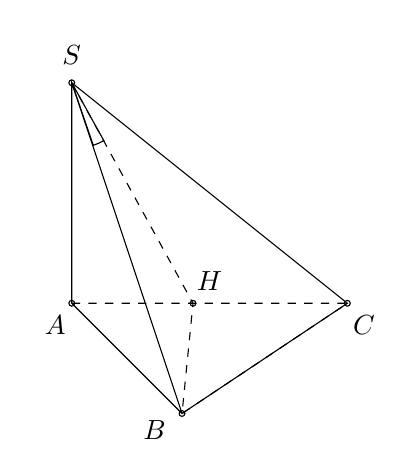
\begin{tikzpicture}[scale=0.7]
				\clip(-0.8,-2.5) rectangle (5.8,5);
				\draw [shift={(0.,4.)}] (0,0) -- (-61:1.2) arc (-61:-71:1.2) -- cycle;
				\draw (0,0)--(2,-2)--(5,0)--(0,4)--(0,0)--(0,4)--(2,-2);
				\draw [dashed] (0,0)--(5,0)--(2,-2)--(2.2,0)--(0,4);
				\draw  (0,0) circle (1.5pt) (-0.3,-0.4) node {$A$} (2,-2) circle (1.5pt) (1.5,-2.3) node {$B$} (5,0) circle (1.5pt) (5.3,-0.4) node {$C$} (0,4) circle (1.5pt) (0,4.5) node {$S$} (2.2,0) circle (1.5pt) (2.5,0.4) node {$H$};
			\end{tikzpicture}
		}
	}
\end{ex}
\begin{ex}%[Huỳnh Đức Vũ, soạn đề cương toán 11-KNTT]%[1H3G3-3]
	Cho hình chóp $S.ABCD$ có $ABCD$ là hình thoi tâm $I$, cạnh $a$, góc $\widehat{BAD}=60^\circ$. Biết $SA=SB=SD=\dfrac{a\sqrt{3}}{2}$. Gọi $\alpha$ là góc giữa đường thẳng $SD$ với $(SBC)$. Tính giá trị $\sin \alpha$.
	\choice
	{$\dfrac{2\sqrt{2}}{2}$}
	{\True $\dfrac{\sqrt{5}}{3}$}
	{$\dfrac{2}{3}$}
	{$\dfrac{1}{3}$}
	\loigiai{
		\immini{
			Xét tam giác $ABD$ ta có $AB=AD=a$; $\widehat{BAD}=60^{\circ}$.\\
			Suy ra tam giác $ABD$ đều cạnh $a$.\\
			Gọi $G$ là trọng tâm tam giác $ABD$.\\
			Suy ra $G$ là tâm đường tròn ngoại tiếp tam giác $ABD$.\\
			Vì $SA=SB=SD$ nên $SG$ là trục của đường tròn ngoại tiếp tam giác $ABD$.\\
			Suy ra $SG \perp (ABCD) \Rightarrow SG \perp DI$.\\
			Mà $AC \perp DI \Rightarrow DI \perp (SAC) \supset SC \Rightarrow DI \perp SC$.
		}{
			\begin{tikzpicture}[>=stealth,line join=round,line cap=round,font=\footnotesize,scale=1]
				\def\r{3}
				\path
				(0,0) coordinate (A)
				(1.5,1.5) coordinate (B)
				($(A)+(4,0)$) coordinate (D)
				($(B)+(4,0)$) coordinate (C)
				($(A)!.5!(D)$) coordinate (M)
				($(B)!.5!(D)$) coordinate (I)
				($(A)!2/3!(I)$) coordinate (G)
				($(G)+(0,3)$) coordinate (S)
				($(S)!(I)!(C)$) coordinate (H)
				($(H)!(D)!(B)$) coordinate (K)
				;
				\draw (S)--(A)--(D)--(C)--(S)--(D)--(H);
				\draw[dashed] (M)--(B)--(A)--(C)--(B)--(D)--(K)--(S)--(I)--(H)--(B)--(S)--(G);
				\foreach \i/\g in {A/180, B/180, C/0, D/0, I/-90, G/160, H/30, K/60, S/90}
				\fill (\i) circle (1.5pt)+(\g:3mm) node {$\i$};
			\end{tikzpicture}
		}
		\noindent
		Dựng $IH \perp SC$ ($H \in SC$).\\
		Suy ra $SC \perp (DIH)$ mà $SC \subset (SBC)$.\\
		Suy ra $(DIH) \perp (SBC)$ mà $(SBC) \cap (DIH) = BH$.\\
		Dựng $DK \perp BH$ ($K \in BH$).\\
		Suy ra $DK \perp (SBC)$ tại $K$.\\
		Suy ra hình chiếu vuông góc của $SD$ lên $(SBC)$ là $SK$.\\
		Suy ra $(SD,(S B C))=(SD,SK)=\widehat{DSK}=\alpha$.\\
		Ta có $$CG=\dfrac{2}{3} AC=\dfrac{2}{3} \cdot 2 AI=\dfrac{4}{3} \cdot \dfrac{a \sqrt{3}}{2}=\dfrac{2 a \sqrt{3}}{3};\,
		SG=\sqrt{SA^2-AG^2}=\dfrac{a \sqrt{15}}{6};\,
		SC=\sqrt{SG^2+GC^2}=\dfrac{a \sqrt{7}}{2}.$$
		Ta có $\triangle HIC \backsim \triangle GSC$ (g-g) $\Rightarrow \dfrac{HI}{GS}=\dfrac{IC}{SC} \Rightarrow HI=\dfrac{IC \cdot GS}{SC}=\dfrac{\dfrac{a \sqrt{3}}{2} \cdot \dfrac{a \sqrt{15}}{6}}{\dfrac{a \sqrt{7}}{2}}=\dfrac{a \sqrt{35}}{14}$.\\
		Xét tam giác vuông $BIH$ ta có $BH=\sqrt{BI^2+IH^2}=\dfrac{a \sqrt{21}}{7}$.\\
		Ta có $S_{\triangle BHD}=\dfrac{1}{2} DK \cdot BH=\dfrac{1}{2} IH \cdot BD \Rightarrow DK=\dfrac{IH \cdot BD}{BH}=\dfrac{a \sqrt{15}}{6}$.\\
		Xét tam giác $SKD$ ta có $\sin \alpha=\dfrac{DK}{SD}=\dfrac{\dfrac{a \sqrt{15}}{6}}{\dfrac{a \sqrt{3}}{2}}=\dfrac{\sqrt{5}}{3}$.
	}
\end{ex}
\begin{ex}%[Huỳnh Đức Vũ, soạn đề cương toán 11-KNTT]%[1H3B3-3]
	Cho hình chóp tam giác đều $S.ABC$ có cạnh đáy bằng $3a$, đường cao $SH=a\sqrt{3}$. Tính góc giữa đường thẳng chứa cạnh bên và mặt đáy của hình chóp.
	\choice
	{$60^{\circ}$}
	{$30^{\circ}$}
	{\True $45^{\circ}$}
	{$75^{\circ}$}
	\loigiai{
		\immini{	
			Ta có $SH\perp(ABC)$ suy ra $HA$ là hình chiếu của $SA$ lên $(ABC)$.\\
			Suy ra $\left(SA;(ABC)\right)=(SA;AH)=\widehat{SAH}$.\\
			Xét $\triangle ABC$ đều ta có $AB=3a\Rightarrow AH=\dfrac{AB\sqrt{3}}{3}=\dfrac{3a\sqrt{3}}{3}=a\sqrt{3}$.\\
			Xét $\triangle SAH$ vuông tại $H$ ta có $$\tan\widehat{SAH}=\dfrac{SH}{AH}=\dfrac{a\sqrt{3}}{a\sqrt{3}}=1\Rightarrow\widehat{SAH}=45^{\circ}.$$
			Vậy góc giữa đường thẳng chứa cạnh bên và mặt đáy của hình chóp bằng $45^{\circ}$.
		}{\begin{tikzpicture}[scale=1, font=\footnotesize, line join=round, line cap=round,>=stealth]
				\path
				(0,0) coordinate (A)
				(1.2,-1.6) coordinate (B)
				(5,0) coordinate (C)
				($(B)!0.5!(C)$) coordinate (M)
				($(A)!2/3!(M)$) coordinate (H)
				($(H)+(0,3.3)$) coordinate (S)
				;
				\draw (S)--(A)--(B)--(C)--cycle (M)--(S)--(B);
				\draw[dashed] (C)--(A)--(M) (S)--(H);
				\foreach \p/\q in {S/90,A/180,B/-90,C/0,H/-90,M/-40}{
					\path (\p) node[shift={(\q:3mm)}]{$\p$};
					\fill[black] (\p) circle (1.0pt);}
	\end{tikzpicture}}}
\end{ex}
\begin{ex}%[Huỳnh Đức Vũ, soạn đề cương toán 11-KNTT]%[1H3B3-3]
	Cho tam giác $ABC$ đều cạnh $a$. Trên đường thẳng vuông góc với mặt phẳng $\left(ABC\right)$ tại $B$ ta lấy điểm $M$ sao cho $MB = 2a$. Gọi $I$ là trung điểm của cạnh $BC$. Tính $\tan$ của góc giữa đường thẳng $IM$ và mặt phẳng $\left(ABC\right)$.
	\choice
	{$\dfrac{\sqrt{2}}{2}$}
	{$\sqrt{2}$}
	{$\dfrac{1}{4}$}
	{\True $4$}
	\loigiai{
		\immini{Ta có $BI$ là hình chiếu vuông góc của $IM$ lên $\left(ABC\right)$.\\
			Khi đó $\left(IM,\left(ABC\right)\right) = \left(IM,BM\right) = \widehat{MIB}$. \\
			Xét $\Delta IBM$ vuông tại $B$ có $\tan \widehat{MIB} = \dfrac{MB}{BI} = 4$.}{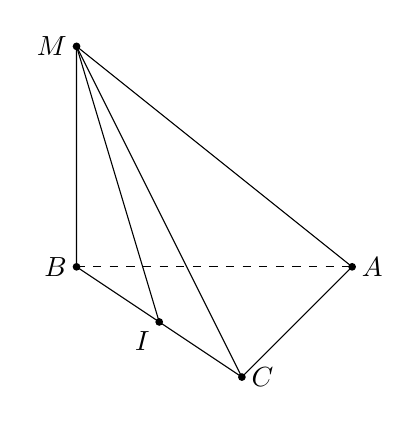
\begin{tikzpicture}[scale=.7]
				\draw (1,0)-- (4,-2)-- (6,0)-- (1,4)--(1,0);
				\draw (1,4)-- (4,-2);
				\draw (1,4)-- (2.5,-1);
				\draw [dashed] (1,0)-- (6,0);
				\fill (1,0) circle (.07) node [left]{$B$};
				\fill (1,4) circle (.07) node [left]{$M$};
				\fill (4,-2) circle (.07) node [right]{$C$};
				\fill (6,0) circle (.07) node [right]{$A$};
				\fill (2.5,-1) circle (.07) node [below left]{$I$};
	\end{tikzpicture}}}
\end{ex}
\begin{ex}%[Huỳnh Đức Vũ, soạn đề cương toán 11-KNTT]%[1H3B3-3]
	\immini{
		Cho hình lăng trụ tam giác đều $ABC.A’B’C’$ có $AB=2$ và $AA’=3$ (tham khảo hình bên). $M$ là trung điểm của $AB$. Góc giữa đường thẳng $MC’$ và mặt phẳng $(ABC)$ bằng
		\choice
		{$90^{\circ}$}
		{$30^{\circ}$}
		{$45^{\circ}$}
		{\True $60^{\circ}$}
	}
	{
		\begin{tikzpicture}[line join=round,line cap=round, font=\footnotesize,scale=1,>=stealth]
			\def \a{3}
			\path
			(0,0) coordinate (A)
			(0:\a) coordinate (C)
			(90:{1.1*\a}) coordinate (A')
			(-60:{0.6*\a}) coordinate (B)
			($(B)+(A')$) coordinate (B')
			($(C)+(A')$) coordinate (C')
			($(B)!0.5!(A)$) coordinate (M);						
			\draw
			(A)--(B)--(C)--(C')--(B')--(A')--(A)(A')--(C')--(B)--(B')
			pic [draw,angle radius=2mm] {right angle = C--A--A'}
			pic [draw,angle radius=2mm] {right angle =B--A--A'};
			\draw[dashed] (A)--(C)--(M)--(C');
			\foreach \x/\g in {A/180,B/180,C/0,A'/180,B'/180,C'/0,M/180}\fill[black] (\x) circle (1pt)+(\g:.3)node{$\x$};
		\end{tikzpicture}
	}
	\loigiai{
		\immini{
			Ta có tam giác $ABC$ đều cạnh $AB=2\Rightarrow\heva{&CM\perp AB\\&CM=\dfrac{AB\sqrt{3}}{2}=\sqrt{3}.}$ \\
			Vì $CC’\perp(ABC)\Rightarrow CC’\perp CM$ hay $CM$ là hình chiếu vuông góc của $C’M$ lên $(ABC)\Rightarrow\left(\widehat{C’M,(ABC)}\right)=\widehat{C’MC}=\alpha $.\\
			Ta có $CC’=A’A=3\Rightarrow\tan\alpha=\dfrac{CC’}{CM}=\dfrac{3}{\sqrt{3}}=\sqrt{3}\Rightarrow\alpha=60^{\circ}$.
		}
		{\begin{tikzpicture}[line join=round,line cap=round, font=\footnotesize,scale=1,>=stealth]
				\def \a{3}
				\path
				(0,0) coordinate (A)
				(0:\a) coordinate (C)
				(90:{1.1*\a}) coordinate (A')
				(-60:{0.6*\a}) coordinate (B)
				($(B)+(A')$) coordinate (B')
				($(C)+(A')$) coordinate (C')
				($(B)!0.5!(A)$) coordinate (M)
				;
				\draw
				(A)--(B)--(C)--(C')--(B')--(A')--(A)(A')--(C')--(B)--(B')
				pic [draw,angle radius=2mm] {right angle = C--A--A'}
				pic [draw,angle radius=2mm] {right angle =B--A--A'} ;
				\draw[dashed] (A)--(C)--(M)--(C') pic [draw,"$\alpha$"] {angle =C--M--C'};
				\foreach \x/\g in {A/180,B/180,C/0,A'/180,B'/180,C'/0,M/180}\fill[black] (\x) circle (1pt)+(\g:.3)node{$\x$};
			\end{tikzpicture}
		}
	}
\end{ex}
\begin{ex}%[Huỳnh Đức Vũ, soạn đề cương toán 11-KNTT]%[1H3K3-3]
	Cho hình chóp $S.ABCD$ có đáy $ABCD$ là hình vuông tâm $O$ cạnh bằng $a$, $SA=a$ và $SA$ vuông góc với đáy. Khi đó $\tan$ của góc giữa đường thẳng $SO$ và mặt phẳng $(SAB)$ bằng	
	\choice
	{\True $\dfrac{\sqrt{5}}{5}$}
	{$\sqrt{2}$}
	{$\sqrt{5}$}
	{$\dfrac{\sqrt{2}}{2}$}
	\loigiai{
		\immini{
			Gọi $H$ là trung điểm của $AB$.\\
			Ta có $OH \perp SA$ ($SA\perp (ABCD)$) và $OH \perp AB$ ($\Delta AOB$ cân).\\
			Suy ra $OH \perp (SAB)$.\\
			Khi đó hình chiếu của $SO$ lên mặt phẳng $(SAB)$ là $SH$.\\
			Khi đó $(SO,(SAB))=(SO,SH)=\widehat{HSO}$.\\
			Xét tam giác $SAH$ vuông tại $A$. $$SH=\sqrt{SA^2+AH^2}=\sqrt{a^2+\dfrac{a^2}{4}}=\dfrac{a\sqrt{5}}{2}.$$
			Xét tam giác $SOH$ vuông tại $H$, ta có
			$$\tan\widehat{HSO}=\dfrac{OH}{SH}=\dfrac{\dfrac{a}{2}}{\dfrac{a\sqrt{5}}{2}}=\dfrac{\sqrt{5}}{5}.$$}
		{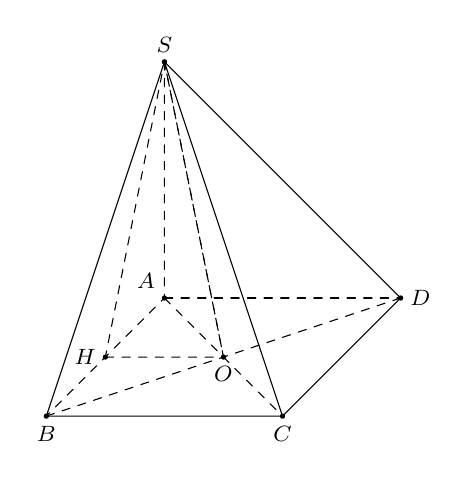
\begin{tikzpicture} [scale=0.75, font=\footnotesize, line join=round, line cap=round, >=stealth]
				\draw[fill=black] (0,0) node[above left] {$A$} circle(1pt);
				\draw[fill=black] (-2,-2) node[below] {$B$} circle(1pt);
				\draw[fill=black] (2,-2) node[below] {$C$} circle(1pt);
				\draw[fill=black] (4,0) node[right] {$D$} circle(1pt);
				\draw[fill=black] (1,-1) node[below] {$O$} circle(1pt);
				\draw[fill=black] (0,4) node[above] {$S$} circle(1pt);
				\draw[fill=black] (-1,-1) node[left] {$H$} circle(1pt);
				\draw (-2,-2)--(2,-2)--(4,0);
				\draw [dashed] (-1,-1)--(1,-1)--(0,4)--(-1,-1);
				\draw [dashed] (0,4)--(0,0)--(-2,-2);
				\draw [dashed] (0,0)--(4,0);
				\draw [dashed] (0,0)--(2,-2);
				\draw [dashed] (-2,-2)--(4,0);
				\draw (-2,-2)--(0,4)--(2,-2);
				\draw (0,4)--(4,0);
				\draw [dashed] (0,4)--(1,-1);
				\path
				(-1,-1)coordinate(H)
				(0,4) coordinate(S)
				(1,-1)coordinate(O)
				(0,0) coordinate(A)
				(-2,-2) coordinate(B);		
			\end{tikzpicture}
		}
	}
\end{ex}
\begin{ex}%[Huỳnh Đức Vũ, soạn đề cương toán 11-KNTT]%[1H3B3-3]
	Cho hình lăng trụ đều $ABC.A'B'C'$ có tất cả các cạnh bằng $a.$ Gọi $G$ là trung điểm của cạnh $B'C.$ Tan của góc giữa đường thẳng $AG$ và mặt phẳng $(ABC)$ bằng
	\choice
	{$\dfrac{\sqrt 2}{2}$}
	{\True $\dfrac{\sqrt 3}{3}$}
	{$\dfrac{\sqrt 3}{2}$ }
	{$\sqrt 3 $}
	\loigiai{
		\immini{Gọi $H$ là trung điểm cạnh $BC.$\\
			Ta có $HG\perp (ABC)$\\
			$\Rightarrow AH$ là hình chiếu vuông góc của $AG$ lên mặt phẳng $(ABC).$\\
			$\Rightarrow\left(AG,(ABC)\right)=\left(AG,AH \right)=\widehat{HAG}=\varphi $.\\
			Mặt khác $\Delta AHG$ vuông tại $H$, có $HG=\dfrac{1}{2}\cdot CC'=\dfrac{a}{2}$, $AH=\dfrac{a\sqrt 3}{2}$ và\\ $\tan\varphi=\dfrac{HG}{AH}=\dfrac{\sqrt 3}{3}.$}{\begin{tikzpicture}[scale=.5]
				\coordinate (A) at (0,0);
				\coordinate (B) at (3,-2);
				\coordinate (C) at (5,0);
				\def\cc{6}
				\coordinate (A') at ($(A)+(0,\cc)$);
				\coordinate (B') at ($(B)+(0,\cc)$);
				\coordinate (C') at ($(C)+(0,\cc)$);
				\coordinate (G) at ($(B')!0.5!(C)$);
				\coordinate (H) at ($(B)!0.5!(C)$);
				\draw(A)--(B)--(C)--(C')--(B')--(A')--(C') (B)--(B') (G)--(H) (B)--(C') (B')--(C) (A)--(A');
				\draw[dashed](A)--(C) (A)--(G) (A)--(H) (A)--(G);
				\foreach \p/\g in {A/180,C/0,B/-90,A'/90,B'/90,C'/90, G/0, H/0}\draw[fill=black] (\p) circle (1pt)node[shift={(\g:.2)},scale=.8]{$\p$};			
	\end{tikzpicture}}}
\end{ex}
\Closesolutionfile{ans}
\begin{indapan}{10}
	{ans/ans-1K7-24-Dang4}
\end{indapan}
